\problemname{Astronomas}
\illustration{.3}{img/TychoBrahe.JPG}{}

\noindent
Astronomo aistra -- stebėti žvaigždes.
Tiksliau, jis patiria neapsakomą malonumą stebėdamas $k$~žvaigždių vienu metu pro teleskopą.
Sukonstruoti teleskopą, kurio spindulys lygus~$r$, kainuoja $t\cdot r$~kronų.
Naujai sukonstruotas teleskopas bus nukreiptas tiesiai į koordinačių pradžios tašką $(0,0)$. 
Nukreipti į kitą tašką taip pat reikalauja pastangų;
nukreipti teleskopą į tašką, esantį atstumu $d$ nuo pradžios taško, kainuoja $s\cdot d$~kronų.
Astronomas gali stebėti visas žvaigždes, nutolusias daugiausiai $r$ nuo taško, 
į kurį nukreiptas teleskopas.

Kiek kainuoja sukonstruoti teleskopą ir nukreipti jį į tokį tašką, kad vienu metu būtų galima stebėti $k$~žvaigždžių?

\medskip

Visos koordinatės ir atstumai skaičiuojami Euklidinėje plokštumoje.


\section*{Pavyzdys}

Čia pateikiamas pavyzdys su $n=3$ žvaigždžių, kurių koordinatės yra $(0,0)$, $(2,0)$ ir $(3,1)$.
Tamsesnis plotas žymi teleskopą, kurio spindulys lygus~$1$ ir kuris nukreiptas į tašką $(1,0)$. Šis teleskopo plotas apima dvi žvaigždes. Tai kainuotų $s + t$~kronų ir tai yra optimalus sprendinys pavyzdinei įvesčiai~$3$ (\emph{sample input~$3$}).
Paveikslėlis taip pat parodo optimalius sprendinius pavyzdinėms įvestims~$1$, $2$ ir $4$ (\emph{sample inputs~$1$, $2$, $4$})).

\medskip
\noindent
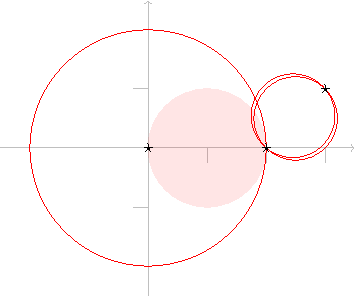
\includegraphics[width=.3\textwidth]{img/samples.pdf}


\section*{Įvestis}

Pirmoje eilutėje pateikti keturi sveikieji skaičiai:
skaičius~$k$, žymintis, kiek žvaigždžių astronomas nori stebėti,
skaičius~$n$, kiek žvaigždžių šiąnakt yra danguje,
teleskopo nukreipimo kaina~$s$ ir
teleskopo konstravimo kaina~$t$.
Tuomet pateiktos $n$ eilučių. $i$-ojoje eilutėje pateikiami du sveikieji skaičiai $x_i$ ir $y_i$ -- 
$i$-osios žvaigždės koordinatės.

\section*{Išvestis}

Išveskite vieną realųjį skaičių: mažiausią kronų sumą, kurią teks astronomui išleisti.

\section*{Ribojimai ir vertinimas}

Visada galios šie ribojimai:
\begin{enumerate}
\item $1\leq k\leq n\leq 700$. % constraint:kn
\item $x_i, y_i\in \{-10^9,\ldots, 10^9\}$ kiekvienam $i\in\{1,\ldots,n\}$. % constraint:xy
\item $s,t\in \{0,\ldots, 10^9\}$. % constraint:st
\item Išvestis laikoma teisinga, jeigu jos ir teisingo atsakymo
reliatyvi arba absoliutinė paklaida yra ne didesnė nei $\epsilon = 10^{-6}$.
\end{enumerate}

Jūsų sprendimas bus testuojamas su keliomis testų grupėmis, kurių kiekviena verta tam tikro skaičiaus taškų.
Kiekviena testų grupė sudaryta iš įvairių testų.
Testų grupės taškai skiriami tik išsprendus visus testus, esančius toje grupėje.
Galutinis rezultatas lygus daugiausiai surinkusio sprendimo taškų skaičiui.

\medskip
\noindent
\begin{tabular}{lll}
  Grupė & Taškai & Papildomi ribojimai\\\hline
  $1$ & $8$ &  $t\leq s$\\
  $2$ & $9$ & $n\le 50$ ir $s=0$\\
  $3$ & $18$ & $s=0$\\
  $4$ & $13$ & $n\leq 50$\\
  $5$ & $14$ & $n\leq 350$\\
  $6$ & $15$ & $\epsilon = 1/10$\\
  $7$ & $23$ & \emph{Jokių papildomų ribojimų}\\
\end{tabular}
